%!TEX root = ../main.tex
%%

\chapter{Design \& Methodology}
Neural network models (specifically CNNs) have previously shown efficacy in cell recognition and counting, so a model of this kind will be the core component of the cell counting artefact. The artefact will process input images and return a reliable count of cells in the image as an output.\\

The project will be evaluated on the following requirements, which are prioritised according to the MoSCoW method. ‘Must’ requirements are essential to the project’s success, and the project’s success will be evaluated on them. ‘Should’ requirements add value to the project beyond its core functionality, but are not essential. ‘Could’ requirements add further value but are the lowest-prioritised, and their implementation should not be attempted unless all higher-priority requirements are implemented and time remains for development.

\section{Requirements}
\subsection{Functional Requirements}
\subsubsection{Must}
\paragraph{As an input, accept an image (or image patch) from the dataset.}
At the least, the artefact should accept input images from the Micropics dataset, or patches thereof. The images in the dataset have a resolution of 1920x1080, so are not usable in a neural network model in their unprocessed form. Some neural networks, like YOLO, accept images of an arbitrary shape and size, but will still subject these images to transformation (e.g. cropping or padding with zeros) in order that they can be processed. These transformations could negatively affect the model’s performance, particularly since the objects to be counted are small. To solve this problem, the images could be segmented into smaller patches that can be processed by the model.

\paragraph{As an output, produce a reliable count of cells in the image.}
This requirement can be evaluated using the ground-truth images in Micropics. The Micropics project includes a script to return a count of the ground-truth dots in an image, so the artefact can be evaluated by the mean absolute error of the artefact’s guesses versus the ground-truth numbers.

\paragraph{Process any valid input without errors}

\subsubsection{Should}
\paragraph{Use the optimal hyperparameters for the model.}
The artefact can only achieve its highest possible performance by using the optimal set of model hyperparameters. This will require extensive testing and trial and error.

\subsubsection{Could}
\paragraph{Produce a secondary output for explanation purposes.}
In anticipation that the user desires (or is entitled to) an explanation of the output of the artefact, it could be designed in such a way as to produce one. This would likely take the form of a copy of the input image with any cells highlighted.

\paragraph{Include a user interface.}
The working artefact in its simplest form is not usable by the layman, but a UI could be developed to make it more useful for lay users.

\subsection{Non-functional Requirements}
\subsubsection{Must}
\paragraph{Use Python for development.}
Python is the default language for machine learning tasks.  Many Python libraries exist for image classification use cases, as well as implementations of neural network models YOLO and Faster R-CNN.

\paragraph{Be trained and tested on the Micropics dataset.}
The Micropics dataset defines the project goal, to count filamentous cyanobacteria cells in images. The dataset may be subject to additional processing, or annotation depending on the model used: for example, the only form of ground truth that YOLOv5 accepts is bounding box annotations around each object to be classified.

\paragraph{Have a corresponding project log.}
This is a requirement of any Honours Project, and will provide a valuable record of the evolution of the project.

\paragraph{Use a capable machine for computation.}
Access to a suitable GPU can be sought from Google Colaboratory or the University.

\paragraph{Be completed by the End of Year Show date.}

\subsubsection{Should}
\paragraph{Use a deep CNN model for detection-based counting of cells (such as Faster R-CNN or YOLO).}
Deep CNN models have previously shown success in the task of detection-based enumeration of cells in images, and implementations of such detection-based models are readily available.

\paragraph{Process an input image quickly at test time.}
Image processing speed is dependent on the model used, but modern localisation networks such as YOLO and Faster R-CNN process images in a trivial amount of time. Processing should not be expected to take more than 1 minute.

\paragraph{Process training data quickly at train time.}
Training time is dependent on the complexity of the model and the training pipeline, so the optimal training parameters (epoch number, batch size etc.) should be found through experimentation. Training time is also dependent on the size of the dataset, so a subset could be used instead of the full dataset. In this case a tradeoff would have to be considered between the size of the dataset used and the model’s performance, since the model will improve with more data.

\paragraph{Be backed up to a version control system.}
To prevent data loss, the project must exist redundantly on a remote repository (likely GitHub).

\paragraph{Be functional by the due date of the Proof of Concept deliverable.}

\subsubsection{Could} 
\paragraph{Use the Pytorch implementation of YOLOv5.}

\paragraph{Use the Keras implementation of YOLOv3 or v4.}

\paragraph{Use Faster R-CNN.}

\subsubsection{Use a density estimation method to count cells.}
Density estimation, rather than detection-based counting, has recently emerged as an alternative method for object counting. This could be explored for comparison with a detection-based method.

\section{Methodology}
\subsection{Legal, Social \& Ethical Issues}
The Micropics dataset is internal to the University and contains no sensitive data, so its use does not present any ethical concerns. In the first instance, the artefact serves as a proof of concept, and is not meant to be used for any safety-critical cell counting application.\\

Inevitably, some count error will be present, but the artefact should ideally err on the side of overcounting rather than undercounting, since false positives are more desirable than false negatives in this case. False negatives might lead to severe consequences for human and animal health, for example if a contaminated water source was determined to be safe, whereas a false positive might inconsequentially be reviewed by a human operator.

\subsection{Data Preparation}
To allow the images in Micropics to be used in training and testing of a neural network, while preventing the destruction of any information in the images by cropping or scaling, the full-resolution images will be split into patches using the \verb|patchRGB.py| utility from the Micropics repository\footnote{GitHub - pamelaajohnston/micropics. (no date). Available at: https://github.com/pamelaajohnston/micropics (Accessed: 05 May 2022).}. Of the 311 images in the Micropics dataset, 20 images each from both the dot-annotated set and the unannotated set will be used. 20 full images was seen as a suitable number for the project because, when split into 224x224 pixel patches, they amount to an acceptably large dataset size of 640 patches while also minimising time spent on the time-consuming and menial annotation process. This allows for a good tradeoff between annotation and experimentation. The patches will be segregated into train, test, and validation sets. Initially the train/test/validation split will be 50/25/25, allowing for experimentation to determine the effect of adding more training data.

\subsection{Data Annotation}
The existing data annotation in Micropics takes the form of a red dot drawn at the centre of each cell. This annotation is incompatible with any detection model including YOLO, so the dataset must be reannotated. The only form of annotation YOLO will accept is edge-aligned rectangular bounding boxes, encompassing each instance of the object(s) to be detected. Several software tools exist for the purpose of annotating images in this way.

\subsubsection{Label Studio}
Label Studio\footnote{Label Studio – Open Source Data Labeling. (no date). Available at: https://labelstud.io/ (Accessed: 21 Apr 2022)} is an open-source data annotation tool widely used in industry. It offers the option to export annotations to many formats, including YOLO. In addition to images, many other types of data can be annotated, including audio and text. Keyboard shortcuts are included for navigation through the dataset, and are based around the WASD configuration, freeing the mouse hand for drawing.\\

Two issues were apparent with Label Studio for the purposes of this project. The one first noticed involved its web-based user interface. During annotation, images are displayed on the page at their actual size and cannot be enlarged. 'Zooming' into the image is possible, but only results in the zoomed image remaining cropped within a box the size of the original image. Since the image patches are 224-pixel squares, they are particularly small on a high-resolution display and this makes annotation difficult (see Figure \ref{label-studio-large}).\\

\begin{figure}[h!]
	\centering
	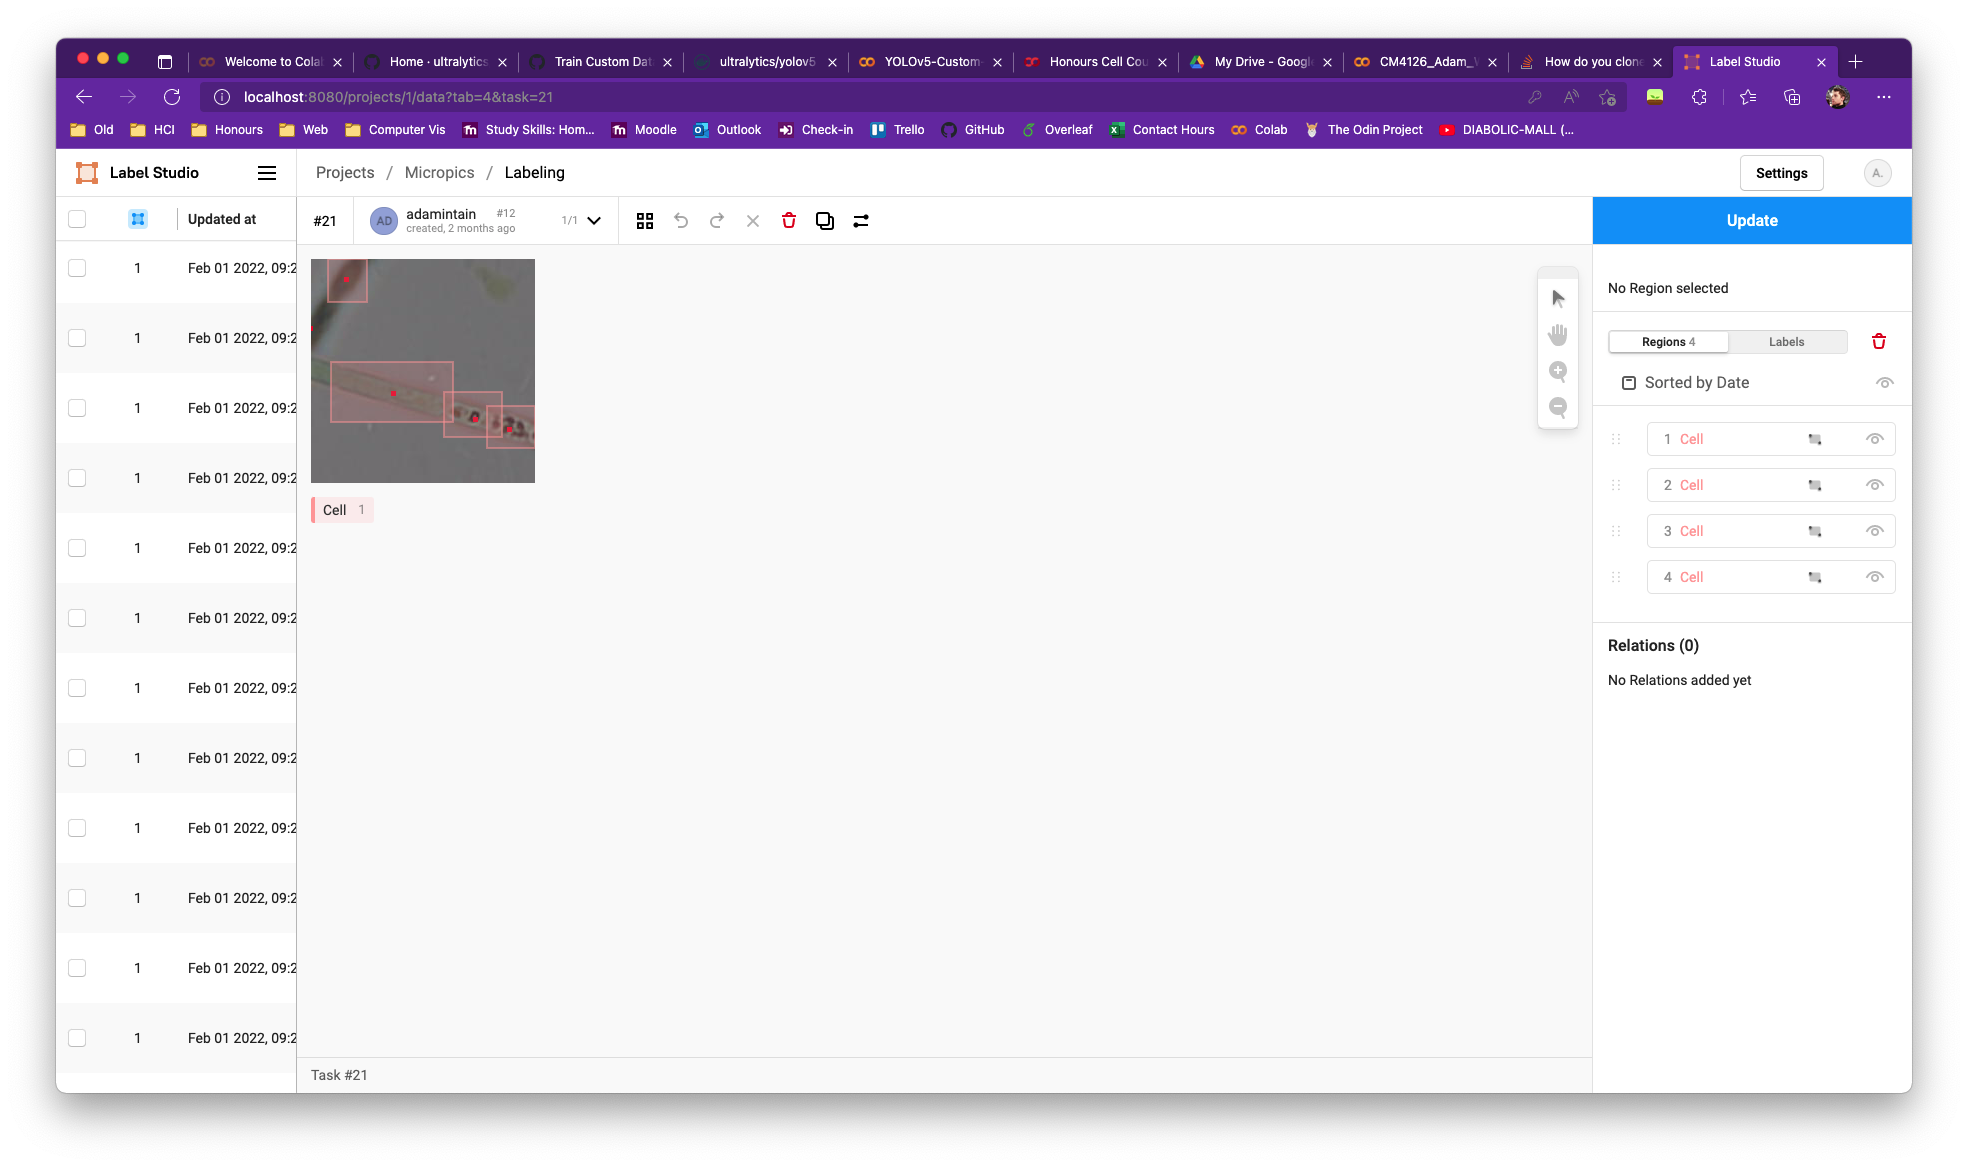
\includegraphics[width=0.8\textwidth]{images/03Design/label-studio-large.png}
	\caption{Label Studio's user interface on a high-resolution display}
    \label{label-studio-large}
\end{figure}

The second feature of Label Studio that made it less suitable for this project was the fact that a sequence of random characters is prepended to the filename of each exported image and label (see Figure \ref{label-studio-prefix}). In this project, the dot-annotated images from the dataset are used for annotation, but the unannotated originals are used in training. The mismatch between image and label filenames means that exported labels cannot be used with the unannotated images without a solution to remove these filename prefixes.

\begin{figure}[h!]
	\centering
	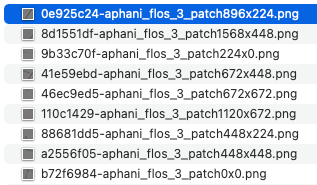
\includegraphics[width=0.5\textwidth]{images/03Design/label-studio-prefix.png}
	\caption{Images annotated by Label Studio with random filename prefixes}
    \label{label-studio-prefix}
\end{figure}

\subsubsection{LabelImg}
LabelImg (see Figure \ref{labelImg}) is another open-source image labeller which exports YOLO-format annotations\footnote{GitHub - tzutalin/labelImg. (no date). Available at https://github.com/tzutalin/labelImg (Accessed: 21 Apr 2022).}. It is an older, better-established tool than Label Studio, with more than double the number of GitHub 'Stars' (17.2k to 8.1k). It is also strictly limited to image annotation.\\

LabelImg was found to be a highly ergonomic tool for navigating and annotating the dataset, which did not suffer from either of the aforementioned issues with Label Studio. In LabelImg, the image being annotated simply grows or reduces with the window size, allowing small images to be 'zoomed' on large displays. Filenames for label files always match the filename of the corresponding image, eliminating the problem of filename mismatch between labels and unannotated images. Some options had to be configured⁠—'Use Default Class Label' and 'Auto Save Mode' were toggled on to prevent object class and save prompts from appearing when drawing a bounding box or moving to a new image⁠⁠—but once these steps were taken, navigating the dataset and drawing bounding boxes was easy, and was streamlined by the presence of WASD-based keyboard shortcuts for dataset navigation, as in Label Studio.

\begin{figure}[h!]
	\centering
	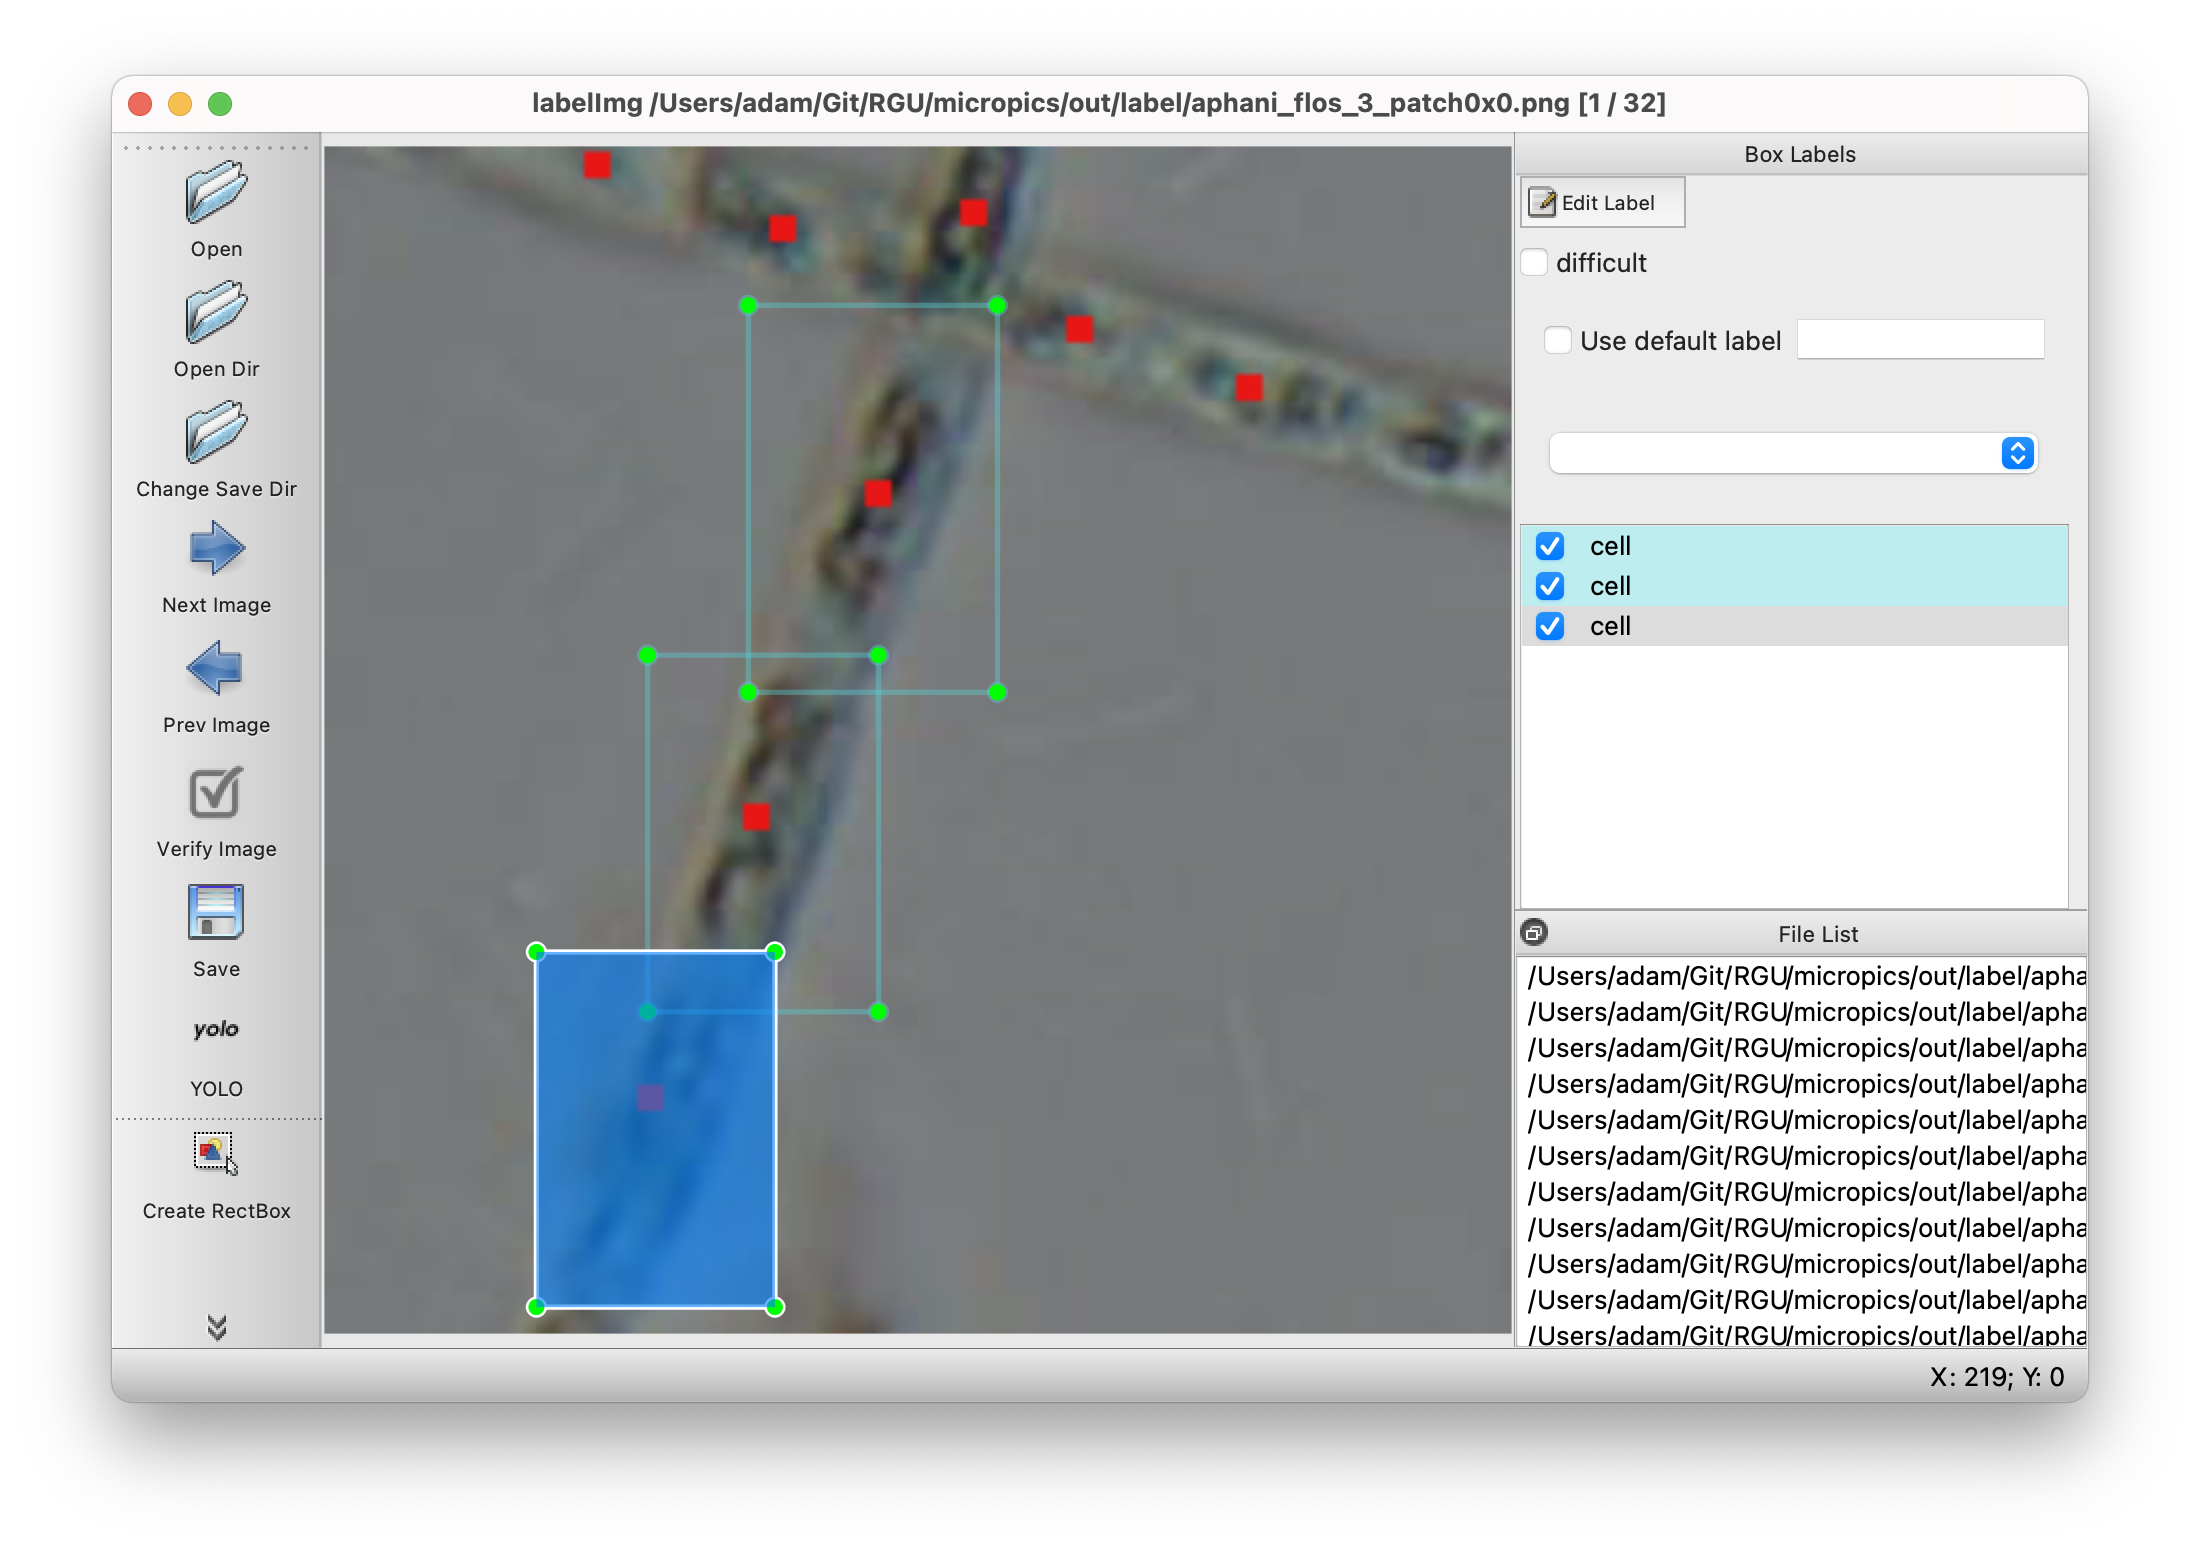
\includegraphics[width=0.8\textwidth]{images/03Design/labelImg.png}
	\caption{LabelImg's user interface}
    \label{labelImg}
\end{figure}

\subsubsection{Annotation Rules}
Annotation presents a particularly significant challenge in the project's methodology. The lack of domain knowledge on the part of the annotator means that even in the dot-annotated images, it is often difficult to distinguish cells in the same trichome from each other. Wherever this significantly affects annotation, it will be taken into account that annotation dots are located at the centre of each cell, and bounding boxes will be drawn around this central dot so as to slightly intersect the bounding boxes on either side.\\

Other cells are difficult to label because they are dot-annotated but out-of-focus, occluded by other cells, or exceeding the edge of the patch. Some ground rules for labelling are required to avoid ambiguity. For the first version of the annotations, in order to be labelled, it will be required that cells are:

\begin{enumerate}
    \item Dot-annotated
    \item In focus
    \item Unoccluded
    \item Wholly visible and not appearing to exceed the edge of the patch
\end{enumerate}

\subsubsection{YOLO Annotation Format}
A dataset in YOLO is defined by a YAML file (e.g. \verb`data.yaml`), which contains the base path to the dataset and the directories of each subset (train, test, validation) relative to this base path (an example can be seen in Listing \ref{yaml}). This file must be created manually, and the dataset must be organised as specified in the file. During training, YOLO will use the YAML file to automatically find corresponding labels for images by looking in the \verb|<database-path>/labels| directory, but filenames for labels must be identical to those of the corresponding images. The YAML file is passed as the \verb|--data| argument when training is run.\\

Label files are in \verb|.txt| format, and list each instance of a labelled object in their corresponding image (an example can be seen in Listing \ref{label}). Each instance comprises the object class, the coordinates of the bounding box centre, and the bounding box's width and height. In addition, a \verb|classes.txt| file, specifying any object classes labelled in the dataset, must reside in any directory containing annotation files. This file is automatically generated by LabelImg.

\begin{lstlisting}[caption={YAML file for the project dataset}, label={yaml}]
path: /content/drive/MyDrive/dataset
train: images/train
val:  images/val
test: images/test

# number of classes
nc: 1

# class names
names: ["cell"]
\end{lstlisting}

\begin{lstlisting}[caption={An image annotation file in YOLO format. From left to right: object class; coordinates of bounding box centre; bounding box width and height}, label={label}]
0 0.781250 0.200893 0.241071 0.187500
0 0.462054 0.285714 0.227679 0.339286
0 0.368304 0.564732 0.218750 0.290179
0 0.267857 0.821429 0.241071 0.312500
\end{lstlisting}

% \begin{figure}[h!]
% 	\centering
% 	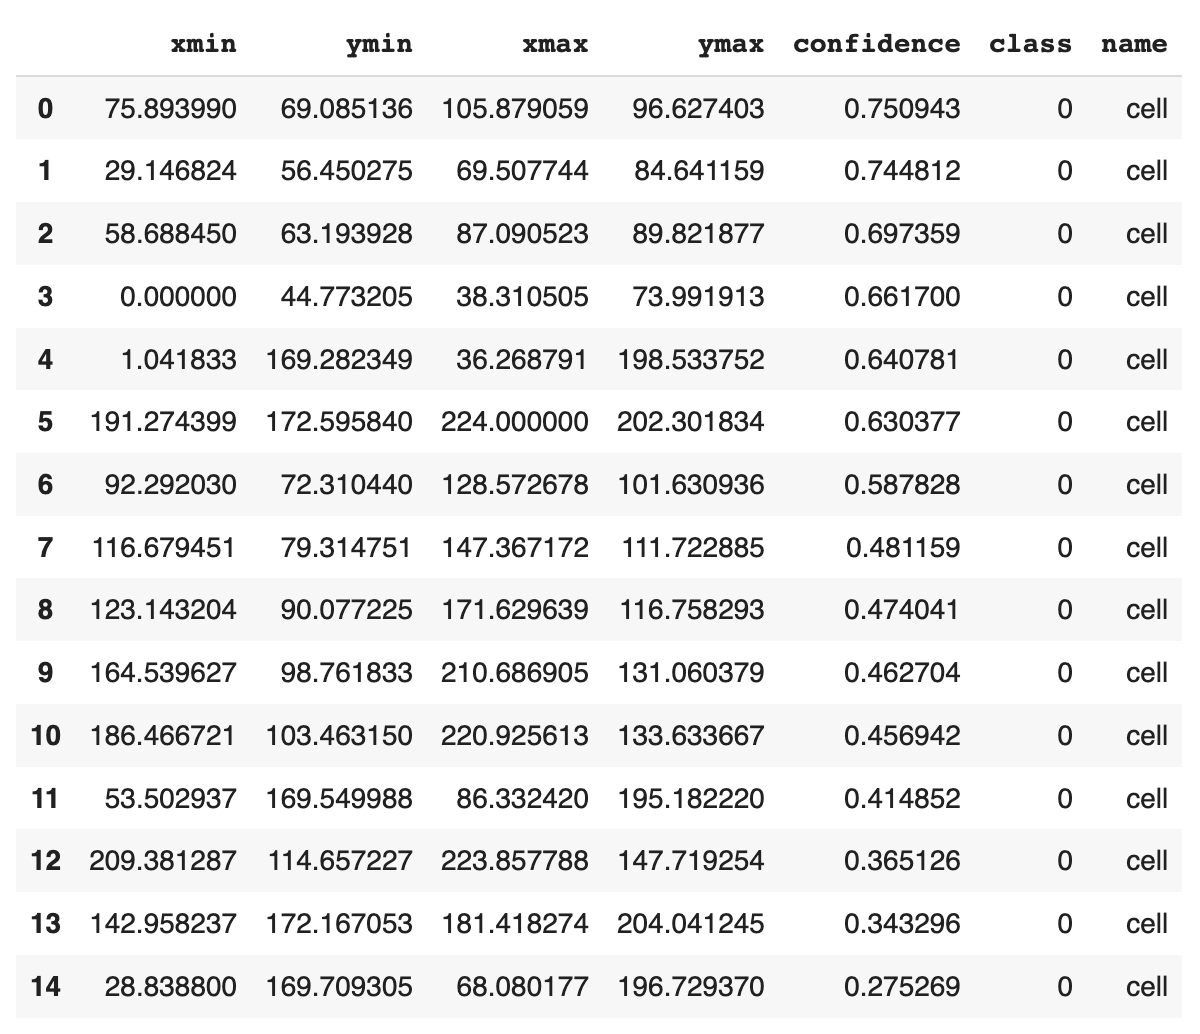
\includegraphics[width=0.8\textwidth]{images/04Implementation/dataframe.png}
% 	\caption{Custom YOLOv5 model's predictions on an image patch from Micropics (DataFrame)}
% \end{figure}

\subsection{YOLO Model}
Many implementations of YOLO exist for both Keras and PyTorch. Some of these are implemented by the community at large, such as a popular implementation of YOLOv3 for Keras\footnote{GitHub - qqwweee/keras-yolo3. (no date). Available at https://github.com/qqwweee/keras-yolo3. (Accessed 22/04/2022).}. Community-developed implementations of YOLO are less reliable than a primary source, since they are maintained by unpaid volunteers and, especially in the case of older YOLO versions, are vulnerable to abandonment. The repository for the aforementioned Keras implementation was last updated on 31 July 2018, and has 477 open issues at the time of writing. Documentation for the repository is also scarce.\\

Ultralytics are the present developers of YOLO in its latest incarnation, YOLOv5. They are the primary source for YOLOv5, which is implemented in PyTorch, and also offer an implementation of YOLOv3 in PyTorch which is in active development. Both of these implementations are offered in their respective GitHub repositories \footnote{GitHub - ultralytics/yolov3. (no date). Available at: https://github.com/ultralytics/yolov3 (Accessed: 05/05/2022).} \footnote{GitHub - ultralytics/yolov5. (no date). Avaliable at https://github.com/ultralytics/yolov5 (Accessed: 05/05/2022).}, and both include a wiki with extensive documentation and tutorials on the network. Compared to a community-maintained YOLO, these qualities of Ultralytics' YOLOv5 make it the better choice as a basis for experimentation.\\

Several pretrained models of varying levels of complexity (see Figure \ref{model_comparison}) are provided with YOLOv5, from YOLOv5n (least complex) to YOLOv5x (most complex), but no pretrained model is suitable for the cell counting use case (see Figure \ref{broc} and Table \ref{yolov5s_counts}), so a custom model must be produced by fine-tuning a pretrained model using the project dataset. Any of the pretrained models can be used as a basis for fine-tuning, so the effects of using different pretrained models can be appraised. The model chosen for initial experimentation was YOLOv5s. Being the second-smallest network, it allows for exceptionally high training speeds, which is ideal for the testing of different combinations of hyperparameters, annotations, and train/test splits. Later experiments might investigate the effects of using a larger and more complex base model. The fact that YOLOv5s is relatively lightweight may also have implications for this use case: the cell counter artefact might be deployed in deprived or rural areas with limited access to clean water, and where human experts are unavailable. In this case it might be deployed on less capable hardware with little or poor networking, and a less complex, more portable model would be desirable in this case.

\begin{figure}[h!]
	\centering
	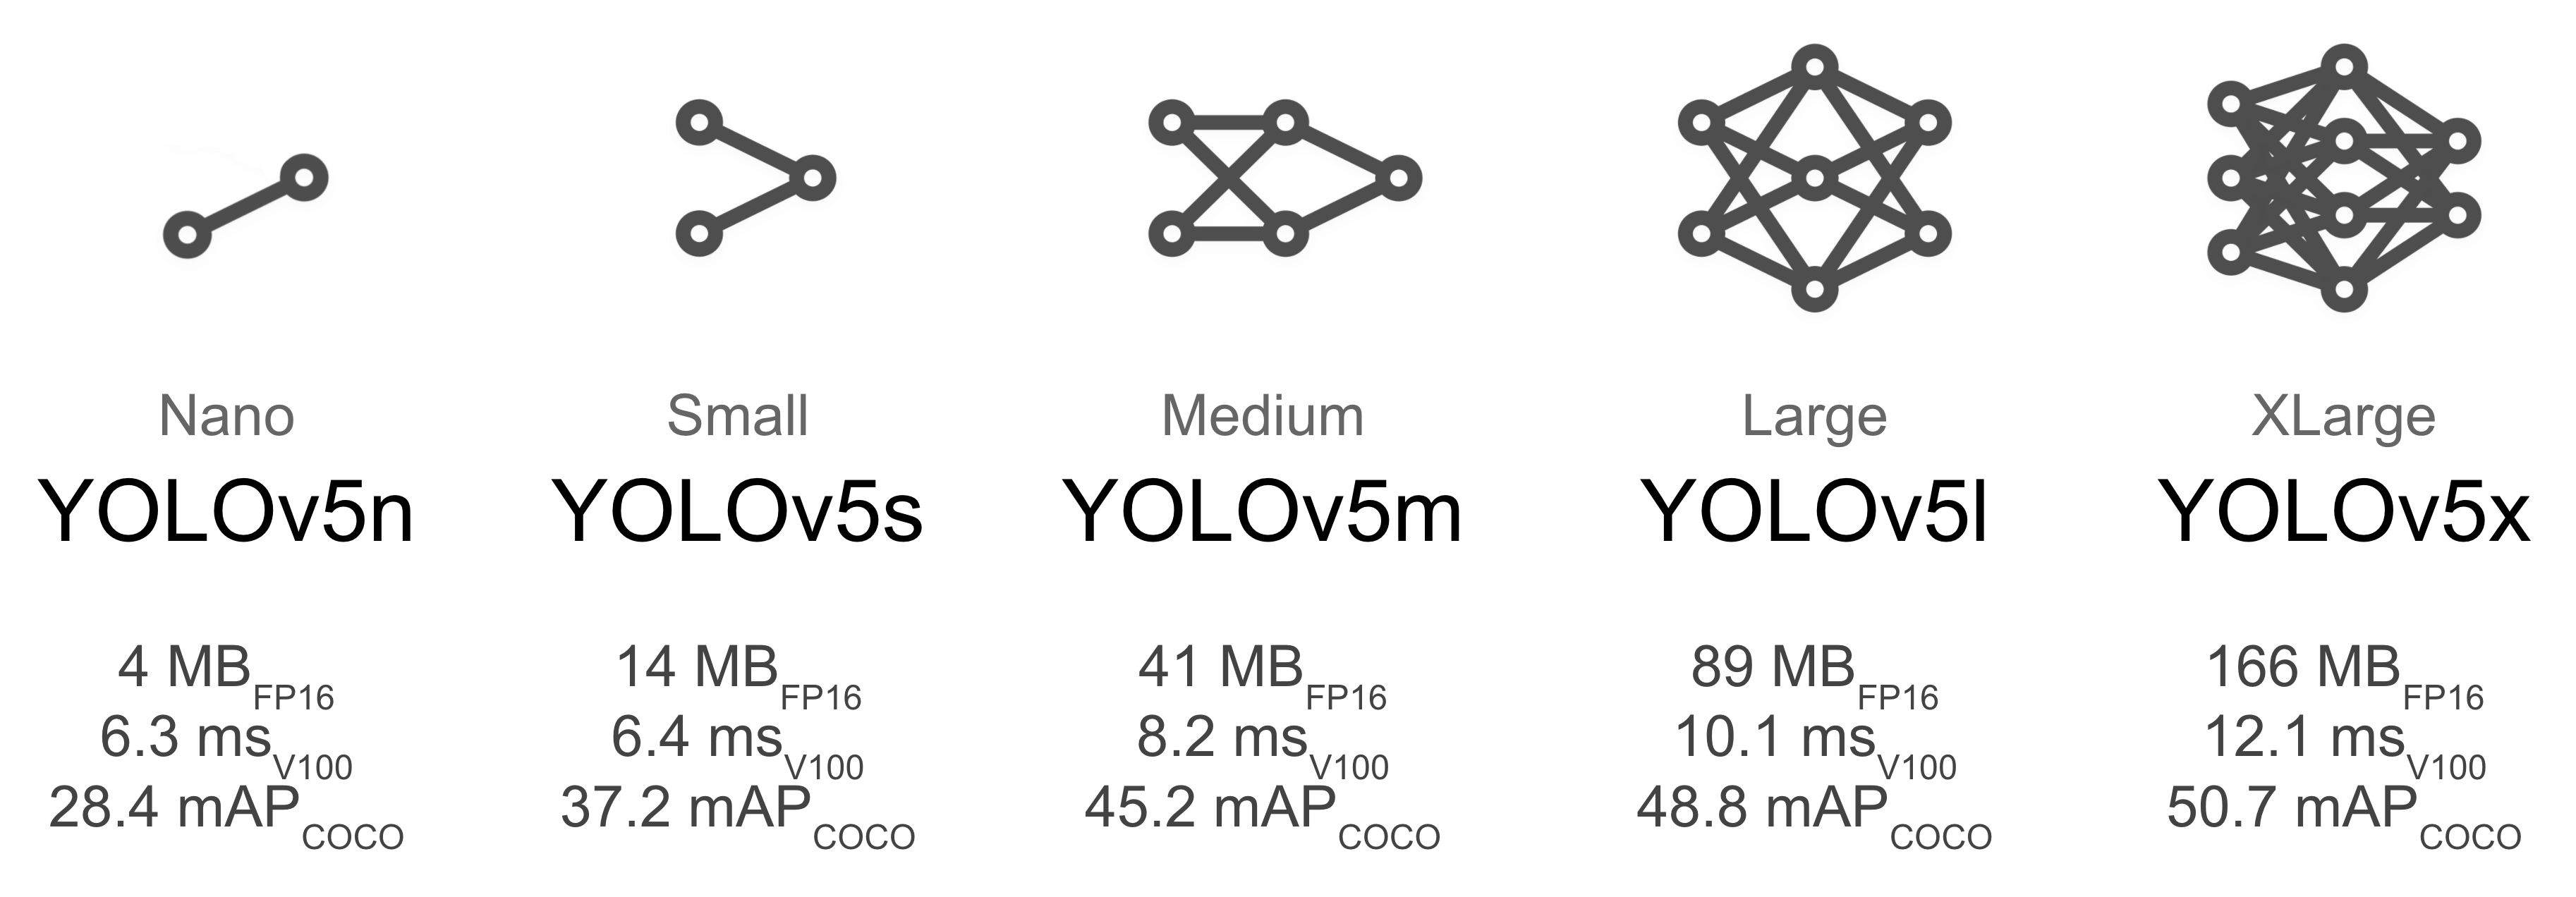
\includegraphics[width=0.8\textwidth]{images/04Implementation/model_comparison.png}
	\caption{Pretrained YOLOv5 models}
    \label{model_comparison}
\end{figure}

\begin{figure}[h!]
	\centering
	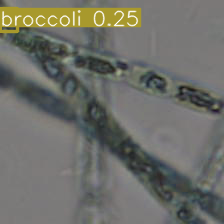
\includegraphics[width=0.5\textwidth]{images/03Design/broc.png}
	\caption{Bounding box predictions on a patch from the test set using YOLOv5s}
    \label{broc}
\end{figure}

\begin{table}
\centering
\begin{tabular}{ |l||l|l|l|l|  }
\hline
\multicolumn{5}{|c|}{Count Error} \\
\hline
Image & Ground Truth & Model Count & Num. Error & Pct. Error \\
\hline
37 &            81 &            1 &          80 &   98.765432 \\
39 &            58 &            3 &          55 &   94.827586 \\
41 &            86 &            0 &          86 &  100.000000 \\
44 &           102 &            0 &         102 &  100.000000 \\
\hline
\end{tabular}
\caption{Count error using YOLOv5s}
\label{yolov5s_counts}
\end{table}

% \begin{table}[h!]
% \centering
% \begin{tabular}{||c c c c c||} 
% \hline
% Image &  Ground Truth &  Model Count &  Num. Error &    \% Error \\
% \hline\hline
% 37 &            81 &            1 &          80 &   98.765432 \\
% 39 &            58 &            3 &          55 &   94.827586 \\
% 41 &            86 &            0 &          86 &  100.000000 \\
% 44 &           102 &            0 &         102 &  100.000000 \\
% \hline
% \end{tabular}
% \caption{Predictions on test set images from Micropics using YOLOv5s (counts)}
% \label{table:1}
% \end{table}

\subsection{Computation Platform}
While YOLOv5 is a fast network, it would be optimal for experiments to be run on a specialised platform for computation-heavy tasks. Multiple runs of training with varying hyperparameters can be dramatically accelerated by GPU computation.

\subsubsection{University DGX}
The first option for computation appraised was the University's Nvidia DGX server. This would provide high throughput and require no monetary investment, so was seen as a desirable option. Upon further investigation, it was found that setting up the DGX to serve a Jupyter Notebook for computation was difficult, and seemed to be obstructed by issues with the machine. Some time was spent identifying the issue before it was tentatively pinpointed as another user appropriating all GPUs. In addition, the outdated CUDA library present on the machine meant that the latest Tensorflow and Jupyter versions could not be installed, resulting in a reliance on older code. At this point the DGX-based approach was abandoned.

\subsubsection{Google Colaboratory}
Google Colaboratory (Colab)s\footnote{Colaboratory. (no date). Available at https://colab.research.google.com (Accessed: 22/04/2022).} provides free and premium access to GPU computation and a Jupyter Notebook environment. Notebooks are stored in the cloud via Google Drive and accessed through a web-based user interface. Google Drive integration also allows datasets to be stored in the cloud along with notebooks, providing a safe storage solution to prevent loss of either code or data during experimentation. Colab offered a harmonious and exceptionally easy-to-use alternative to setting up a computation environment from scratch, where all elements would need to be configured separately and connected.\\

Colab provides a free tier of access to GPU computation, but this is limited and liable to run out during long tasks. A Colab Pro subscription (£8.10 per month) provides more lenient access to computation. Based on its ease of use, web-based nature, and integration with cloud storage, it was decided that Colab represented the best option for the project's computation environment.

\subsection{Evaluation}
The artefact can be straightforwardly evaluated by its counting error, but this should take into account that a consistently overcounting artefact is more desirable than an undercounting one. YOLOv5 also produces various metrics for the model's detection and localisation performance, and these should also be evaluated.\\

For evaluation purposes, it is essential to keep a record of model performance—preferably with detailed results and metrics for each experiment—and to keep the resulting models backed up. Due to the volatile nature of a Colab runtime, any result of a YOLO training experiment, including the model, will be lost when the runtime is disconnected. Measures should be taken to prevent this. YOLOv5 features integration with 'MLOps' platform Weights and Biases\footnote{Weights & Biases – Developer tools for ML. (no date). Available at: https://wandb.ai/site (Accessed: 05/05/2022).}. Once logged in, W\&B automatically detects YOLOv5 training runs, keeps track of all metrics, and saves them to the cloud along with the resulting model. This replaces the otherwise burdensome and risky strategy of extracting models and metrics manually from the Colab runtime, so it was decided W\&B would be used for the purposes of this project. W\&B also presents this data in a user-friendly format (see Figure \ref{wandb}), generating graphs and images to explain otherwise opaque data about the model's performance.

\begin{figure}[h!]
	\centering
	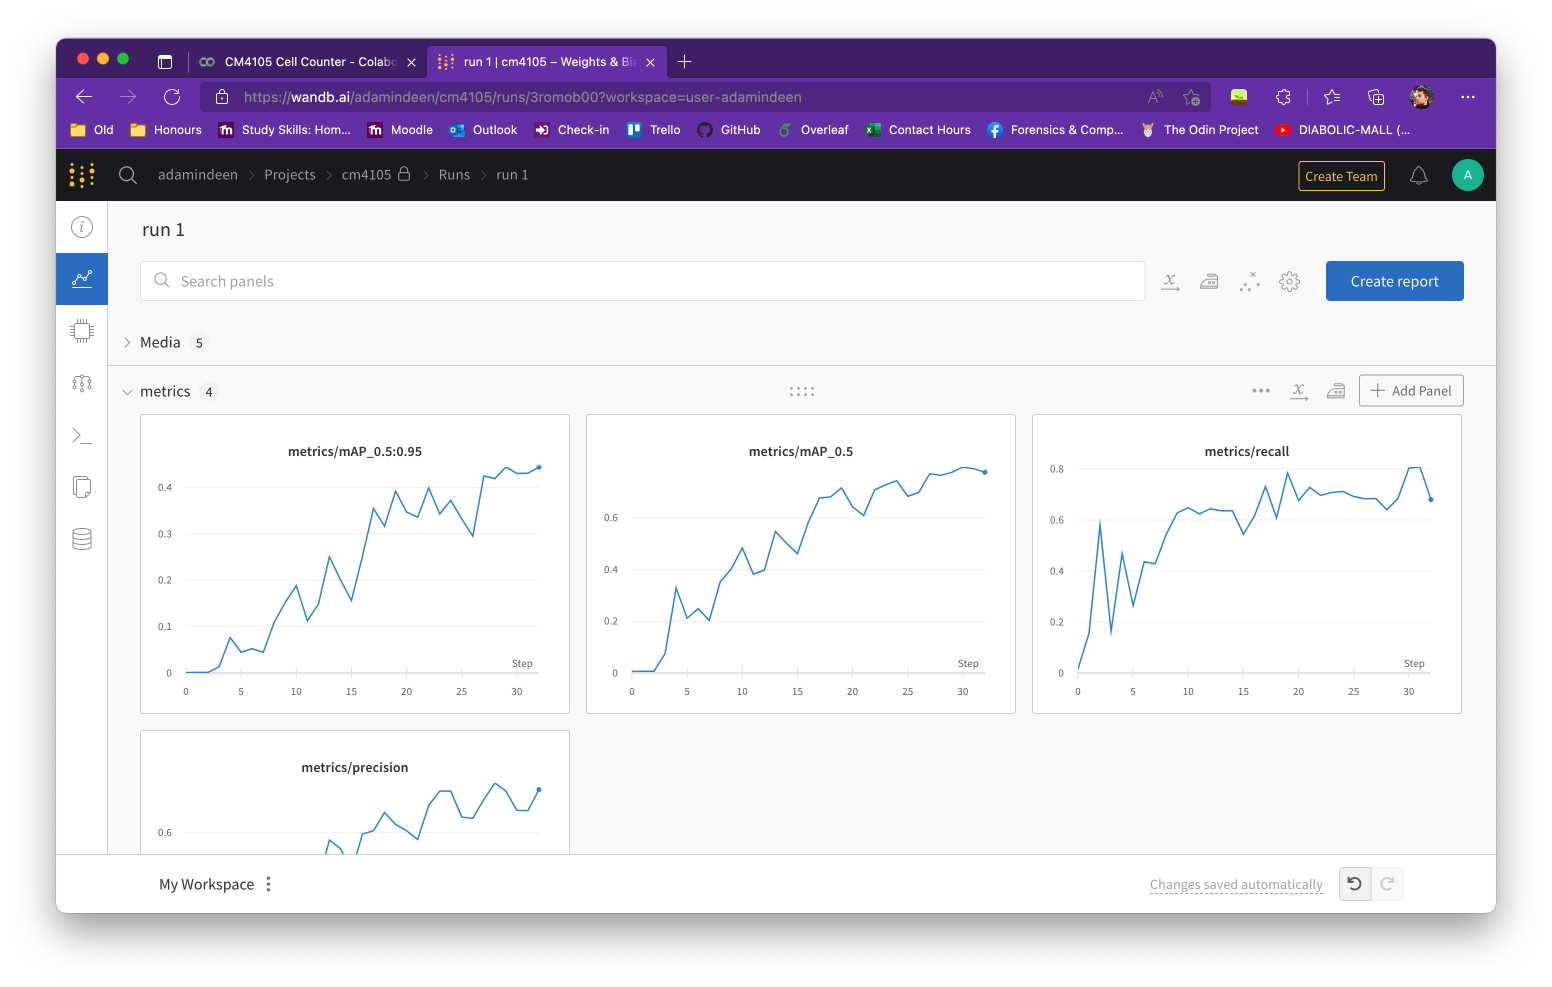
\includegraphics[width=0.8\textwidth]{images/03Design/wandb.png}
	\caption{Weights and Biases' user interface}
    \label{wandb}
\end{figure}

\label{chap:chapter3}

